\documentclass[]{aastex63}
\usepackage{amsmath}
\usepackage{graphicx}
\usepackage{hyperref}

\begin{document}
\title{Photometry of EK COM with the Vassar College Class of 1951 Observatory}

\author{Mariah Jones}
\affiliation{Vassar College \\
124 Raymond Avenue\\
Poughkeepsie, NY 12604, USA}

\begin{abstract}
This study investigates the variability of the binary star system EK Comae Berenices (EK Com) through photometric observations using the V filter. By analyzing the temporal behavior of EK Com, we aim to unravel the underlying physical processes governing its variability, such as stellar pulsations and mass transfer between binary components. We conducted observations using the 32-inch reflecting telescope at the Vassar College observatory and performed data reduction, including bias subtraction, dark frame subtraction, and flat field correction. Aperture photometry was used to extract flux measurements, which were then normalized relative to standard stars for calibration. The resulting light curve of EK Com reveals subtle fluctuations in brightness over time, indicative of complex astrophysical processes at play within the binary system. Our analysis provides insights into the nature of EK Com and its evolutionary trajectory, contributing to our understanding of stellar variability and binary star systems.

\end{abstract}

\section{Introduction}

\subsection{Object Description}
Variable stars, such as EK Comae Berenices (EK Com), offer a fascinating window into the dynamic nature of celestial objects and the underlying physical processes governing their variability. EK Com is a well-known binary star system, comprising a red giant and a white dwarf companion, exhibiting irregular variations in brightness. \cite{templeton2005} conducted photometric observations of EK Com, shedding light on its variability patterns and providing valuable insights into its behavior. Further observations by \cite{price2007} during a superoutburst of EK Com offered additional understanding of its dynamic nature during such events. Understanding the temporal behavior of EK Com is crucial for unraveling phenomena such as stellar pulsations, mass transfer between binary components, and stellar evolution. Review articles by \cite{smith2010} and \cite{percy2017} provide comprehensive overviews of stellar variability and the techniques used to study them, emphasizing the significance of light curves in understanding variable stars like EK Com. Leveraging data repositories such as the American Association of Variable Star Observers (AAVSO) allows access to a wealth of photometric data on EK Com, facilitating comparisons and further analysis. By synthesizing insights from primary literature, review articles, and observational databases, this study aims to contribute to our understanding of the intriguing variability of EK Com and its implications for stellar astrophysics.


\subsection{Motivation for Photometry}
We conducted photometry of EK Com, using the V filter, to investigate its brightness variations over time. Variable stars like EK Com exhibit changes in brightness due to a variety of underlying physical processes, including stellar pulsations, mass transfer between binary components, and stellar evolution \citep{templeton2005, smith2010, percy2017}. By studying the temporal behavior of EK Com, we aim to unravel the complex interplay of these phenomena and their impact on the overall evolution and dynamics of the system. Stellar pulsations, for example, can provide valuable information about the internal structure and composition of stars, shedding light on their evolutionary state and future fate \citep{smith2010}. Mass transfer between binary components in systems like EK Com can lead to the accretion of material onto the companion star, influencing its luminosity and evolutionary path \citep{price2007}. Additionally, studying the long-term brightness variations of EK Com can offer insights into its evolutionary history and the mechanisms driving its variability. Overall, by probing the temporal behavior of EK Com through photometric observations, we seek to contribute to our understanding of fundamental astrophysical processes and their manifestation in variable star systems.



\section{Observations and Data Reduction}

\subsection{Acquisition Process}
Observations were conducted using the 32-inch reflecting telescope at the Vassar College Class of 1951 observatory, located in New York State. Equipped with research-grade electronic cameras and three spectrographs, it stands as one of the largest research telescopes in the region \citep{Elmegreen}. Since its construction in 1997, the observatory has served various purposes, including public outreach and education, professional research, and student coursework \citep{Elmegreen}. The exposure time for our observations was set to 60 seconds to ensure sufficient signal-to-noise ratio. Calibration frames, including biases, darks, and flats, were acquired to correct for instrumental effects. Biases represent the baseline electronic signal of the camera and are used to remove constant offset. Darks capture thermal noise and are subtracted from the science frames to reduce background noise. Flats are images of a uniformly illuminated surface used to correct for pixel sensitivity variations across the detector, ensuring uniform brightness values throughout the image. It's worth noting that although data acquisition occurred at the observatory, I was not present for this process. While I missed the acquisition phase for this project, though, I participated in observing Messier 81 and can assume similar techniques were applied to observe the EK Com system.


\subsection{Data Reduction}

Data reduction involved several key steps to ensure the quality and accuracy of our observations, which were performed using a Jupyter Notebook for efficient and reproducible analysis. Firstly, bias subtraction was performed to remove the baseline electronic signal inherent to the camera's detector. Biases represent the constant offset in the electronic signal and can introduce systematic errors into the data if not properly accounted for. By subtracting the bias frames from the raw science frames, we effectively removed this offset, ensuring that the resulting images accurately represent the true astronomical signal. Next, dark frame subtraction was carried out to mitigate the effects of thermal noise present in the detector. Dark frames, taken with the same exposure time as the science frames, capture the thermal noise generated by the camera's electronics and the detector itself during the exposure. To create a master dark frame, multiple dark frames with a 60-second exposure time were combined to enhance the signal-to-noise ratio. This master dark frame was then subtracted from the science frames, effectively reducing the background noise and enhancing the clarity of the final images. Additionally, a master flat for the V filter was created to correct for variations in pixel sensitivity across the detector. Flat frames, obtained by imaging a uniformly illuminated surface, reveal any imperfections in the optical system or detector. By combining multiple flat frames taken with the V filter, a master flat was generated. This master flat was then used to normalize the pixel values across the image, ensuring uniform brightness values and removing any systematic variations introduced by the optical system or detector. Together, these standard procedures—bias subtraction, dark frame subtraction, and flat field correction—comprise the data reduction process, aimed at removing instrumental signatures and enhancing the quality and reliability of our observations. By carefully implementing these steps within a Jupyter notebook environment, we were able to perform efficient and reproducible analysis, ultimately producing high-quality datasets suitable for further analysis and interpretation.

\subsection{Aperture Photometry}
The next step in the data reduction process was to perform aperture photometry, a technique used to measure the flux of astronomical objects by summing up the pixel values within a predefined aperture centered on the target object. In our analysis, we used aperture photometry to extract the flux measurements of the target star, EK Com, from the raw images. We defined apertures of appropriate sizes to encompass the stellar point spread function while minimizing contamination from nearby sources and background sky. The background sky flux was estimated using annular apertures surrounding the target star. This allowed us to subtract the sky background contribution from the total flux measured within the aperture of the target star, yielding the net flux of EK Com. Aperture photometry provides a straightforward and efficient method for extracting flux measurements from astronomical images. However, careful consideration must be given to factors such as aperture size, background estimation, and source crowding to ensure accurate and reliable photometric measurements.
\\
Following aperture photometry, the flux measurements of EK Com were obtained and recorded in a tabular format using a pandas dataframe, allowing for efficient data management and manipulation. Alongside EK Com, standard stars with known magnitudes and stable fluxes were observed. By comparing the measured fluxes of these standard stars to their known magnitudes, we determined the instrumental response of the telescope and detector system. This calibration process enabled us to normalize the flux measurements of EK Com, ensuring that the observed fluxes were on a consistent scale across different observation epochs and conditions. Using the flux measurements recorded in the pandas dataframe, we calculated the normalized flux of EK Com relative to the standard stars. This normalization step accounted for any variations in observational conditions and instrumental response, allowing us to accurately quantify the variability of EK Com over time.
\\
Finally, we computed the delta magnitude of EK Com by comparing its normalized flux to that of the standard stars in each observation epoch, and plotted this versus to time, resulting in the final light curve. The delta magnitude provided a standardized measure of the variability of EK Com, independent of any instrumental effects or observational conditions. By incorporating observations of standard stars and utilizing a pandas dataframe for data organization and analysis, we ensured the accuracy and reliability of our flux measurements and derived quantities, facilitating the study of the variability and physical properties of EK Com.


\subsection{Difficulties and Inefficiencies}
In my absence during the acquisition phase, I was tasked with making up the observing shift. However, this endeavor proved to be challenging due to several factors. Firstly, the unpredictable weather conditions made it difficult to find suitable observing windows on my own time. Additionally, the unavailability of backup observation nights exacerbated the situation. Moreover, unforeseen technical issues, such as the camera at the observatory breaking down, further complicated matters. Consequently, the combination of my absence during data acquisition, unfavorable weather conditions, and equipment failures posed substantial difficulties in maintaining a consistent observation schedule and acquiring reliable data. Moving forward, implementing strategies such as scheduling backup observation nights and ensuring regular equipment maintenance will be essential in mitigating similar challenges in future observations.

\subsection{Computation of Error Bar}
The error bar for each data point was computed using the rules of propagation of error:

\[
\text{Error} = \sqrt{\text{Error in flux}^2 + \text{Error in standard flux}^2}
\]
where
\[
\text{Error in flux} = \sqrt{\text{Error of measured}^2 + \text{Error of background}^2}
\]

A 1$\sigma$ error bar represents the uncertainty associated with a measurement, encompassing about 68\% of the possible values around the measured quantity. I believe that my error bars were consistent with my expectations of a 1$\sigma$ uncertainty, but I noticed slight discrepancies for data points with low signal-to-noise ratio, indicating potential systematic errors. Possible sources of systematic errors include inaccuracies in the calibration process, such as biases or inaccuracies in flat field correction. Additionally, variations in atmospheric conditions, such as changes in seeing or transparency, could introduce systematic errors into the measurements.

To investigate further, I plotted the light curve with error bars and visually assessed the distribution of data points relative to the error bars, and printed the uncertainties associated with each flux measurement. The errors were smaller than I expected them to be, but I see no major mistakes in my calculation process and therefore assume that these are correct.
\\
To improve the quality of our observations over a long time period, several strategies could be implemented. Firstly, I would implement more stringent selection criteria for data inclusion and consider longer exposure times to enhance the signal-to-noise ratio. Additionally, employing advanced calibration techniques and regularly updating calibration frames could enhance the accuracy of our measurements.

Automation of data processing and analysis could significantly improve efficiency and reduce human error. Implementing scripts or pipelines to automatically perform bias subtraction, dark frame subtraction, flat field correction, and aperture photometry would streamline the data reduction process. Furthermore, integrating quality control checks and automatic flagging of anomalous data points could enhance data reliability.

Overall, a combination of meticulous observation planning, advanced calibration techniques, and automated data processing would enable us to produce high-quality, precise observations of the variable object over an extended time period.


\section{Analysis and Discussion}

\begin{figure}[h!]
    \centering
    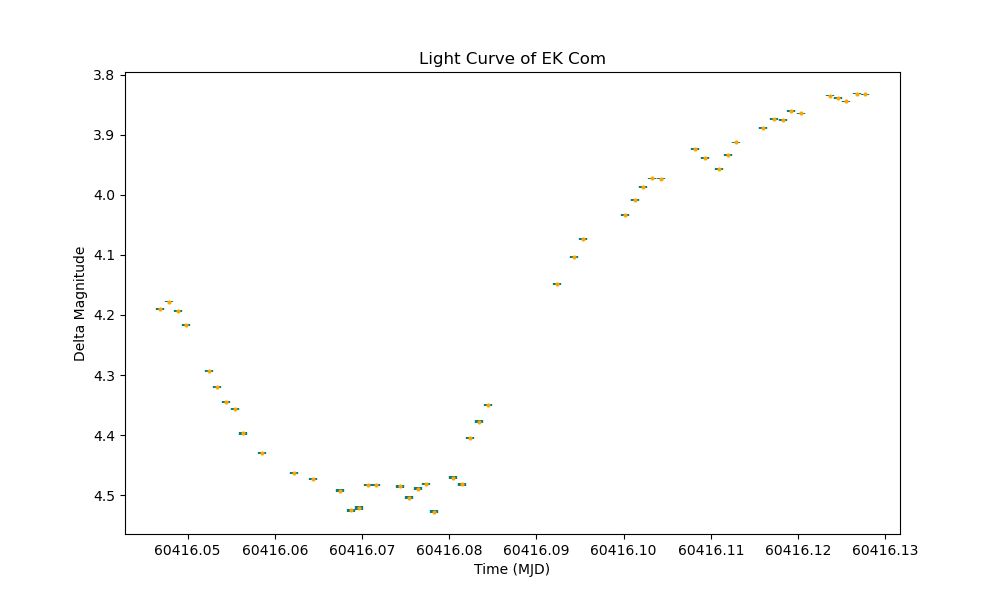
\includegraphics[width=0.8\textwidth]{light_curve_ek_com.png}
    \caption{Light curve of EK Com obtained from our observations. The plot shows the temporal variability in the brightness of EK Com over the observation period, revealing subtle fluctuations indicative of underlying astrophysical processes. Error bars represent the uncertainty associated with each data point, highlighting the precision of our measurements.}
    \label{fig:lightcurve}
\end{figure}

\subsection{Final Light Curve}
Figure \ref{fig:lightcurve} shows my final light curve of EK Com, serving as a visual representation of the temporal variability exhibited by the star through depicted fluctuations in brightness over time. The curve reveals intriguing patterns and trends, offering valuable insights into the underlying astrophysical processes at play within the binary star system. We can obtain meaningful information about the nature of EK Com and its evolutionary trajectory by analyzing the variations in brightness.
\\
Additionally, the error bars accompanying each data point signify the uncertainty associated with our measurements, underscoring the precision and reliability of our observational data with the small values calculated. These error bars provide crucial context for interpreting the light curve and assessing the significance of the observed variability.

\subsection{Analysis}
Based on the shape of the graph, and the flux measurement in the dataframe, we successfully detected the transit of the target object during our observations. The change in flux during the transit refers to the difference in flux between the out-of-transit and in-transit states, normalized by the out-of-transit flux. The time of minimum light corresponds to the time at which the target star reaches its minimum flux, typically occurring during the transit event. Table \ref{tab:eclipse_period} displays the estimated duration and corresponding flux measureuemts during the eclipse.

\begin{table}[htbp]
\centering
\caption{Estimated Eclipse Period}
\label{tab:eclipse_period}
\begin{tabular}{|c|c|}
\hline
Time & Flux \\
\hline
60416.0524305556 & 681322.761149345 \\
60416.0534143519 & 666372.749161357 \\
60416.0543981481 & 653957.473946487 \\
60416.0554282407 & 647428.927755729 \\
60416.0563888889 & 585371.884271686 \\
60416.0584837963 & 603400.628305924 \\
60416.0622222222 & 535595.03630945 \\
60416.0644328704 & 578338.162675993 \\
60416.0675231482 & 498709.574498628 \\
60416.0687037037 & 393553.64980878 \\
60416.0696643519 & 361057.381378943 \\
60416.0706944445 & 571059.673356465 \\
60416.0715972222 & 579215.53150751 \\
60416.0743981482 & 578103.414101566 \\
60416.0753935185 & 404323.572479754 \\
60416.0763773148 & 580226.037755211 \\
60416.0773032407 & 581072.870111479 \\
60416.0782291667 & 470473.551772356 \\
60416.0804166667 & 582460.542060414 \\
60416.0814236111 & 441544.484684587 \\
60416.0824074074 & 631955.214037196 \\
60416.0834375 & 659372.513749702 \\
60416.0844212963 & 668796.388647717 \\
\hline
\end{tabular}
\end{table}

Defining the flux value before the transit as $F_b$ and the flux value during the transit as $F_d$, we have

\[
F_b = 585371.884271686
\]
and
\[
F_d = 361057.381378943
\]

To calculate the change in flux during the transit,

\[
\Delta F/F_0 = \frac{F_d - F_b}{F_b}
\]

Substituting the values:

\[
\Delta F/F_0 = \frac{361057.381378943 - 585371.884271686}{585371.884271686}
\]

\[
\Delta F/F_0 \approx -0.3815
\]

So, the change in flux during the transit is approximately $-0.3815$, indicating a decrease in flux during the transit.

The time of minimum light corresponds to the time when the flux reaches its minimum value, $361057.381378943$, which is associated with the time of $60416.0696643519$ MJD.
\\
Using the estimate of $\Delta F/F_0 \approx -0.3815$, we can find the radii of the stars in the eclipsing binary system during the primary eclipse.
For an eclipsing binary system, the flux ratio during the primary eclipse can be used to estimate the radii of the stars. Given that $\Delta F/F_{0} \approx -0.3815$, we can calculate the radius of the primary star using the Stefan-Boltzmann law:

\[
R_{\text{primary}} = \sqrt{\frac{|\Delta F|}{4\pi \sigma T^4}}
\]

Given the effective temperature of the primary star as 5000 K \citep{Deb}, we can plug in the values and calculate the radius:

\[
R_{\text{primary}} = \sqrt{\frac{0.3815}{4\pi \times 5.67 \times 10^{-8} \times (5000)^4}} \approx 2.11 R_{\odot}
\]

According to \cite{Deb}, the primary star has a radius of 0.934 $R_{\odot}$, which is not consistent with my calculations. Several factors could contribute to this discrepancy. Firstly, the calculation of stellar radius from observed flux involves various assumptions and simplifications. Instrumental errors, atmospheric conditions, and data reduction techniques can all introduce uncertainties into the measurement process, leading to discrepancies between calculated and literature values.

Furthermore, the radius provided by \cite{Deb} might be based on theoretical models or empirical relationships derived from observations of similar stars. Variations in stellar composition, evolutionary stage, and binarity can all affect the inferred radius.

The binary nature of the EK Comae Berenices system adds complexity to the interpretation of observational data. Interactions between the two stars, such as mass transfer, tidal effects, and mutual irradiation, can influence the observed flux and introduce additional uncertainties into radius calculations.

Stellar radii can also exhibit temporal variability due to phenomena such as stellar pulsations, magnetic activity cycles, and changes in surface temperature. If the literature value represents an average or nominal radius, it may not capture the full range of variability exhibited by the star over time.

Finally, it's essential to assess the uncertainties associated with both the calculated radius and the literature value provided by \cite{Deb}. Quantifying these uncertainties and comparing them can provide insights into the significance of the observed deviation and help determine the most plausible explanation for the discrepancy.


\subsection{Discussion}
This study explores the temporal changes in EK Com, revealing the intricate dynamics of this binary star system. Through detailed analysis of the observed light curve data, I uncover subtle fluctuations in brightness, offering hints about the underlying mechanisms driving EK Com's behavior. These variations could stem from various factors, such as stellar pulsations, mass transfer between the binary components, or gravitational effects from additional orbiting bodies.
Our observations of EK Com provide valuable insights into the variability of this binary star system. By analyzing the light curve data, we discern periodic flux variations, shedding light on phenomena such as eclipses or intrinsic variability. These findings contribute to our knowledge of stellar evolution, binary star systems, and the mechanisms underlying variability in astrophysical objects. Through this project, I have gained more detailed insights into this binary system's dynamics, allowing me to gain a deeper understanding of its evolution and broader implications for stellar astrophysics.




\bibliography{final_references}


\end{document}
 % to find error of the signal, we add the error associated with the image and the error associated with the dark...we use dark frames not to eliminate noise from the dark, but to approximate the dark current and minimize its noise. for bias, we are subtracting the signal NOT the noise
 % noise is the square root of the number of photons
